\begin{frame}
    \titlepage
\end{frame}

\begin{frame}{logistics}
    \begin{itemize}
        \item CHALLENGE assignment --- take-home portion of the final
        \item next class --- final exam review
    \end{itemize}
\end{frame}

\begin{frame}{CHALLENGE (1)}
    \begin{itemize}
        \item expect to release before Saturday; due by written final
        \item probably complete all but two 
            \begin{itemize}
                \item five of seven or four of six
                \item (waiting for TA feedback to callibrate difficulty) 
            \end{itemize}
        \item similar format to ``attack'' homeworks
            \begin{itemize}
            \item create a program that produces input
            \end{itemize}
        \item you are responsible for figuringout what scenario applies
    \end{itemize}
\end{frame}

\begin{frame}{CHALLENGE (2)}
    \begin{itemize}
        \item some very similar to prior HWs, some not
        \item reference solutions to OVER, ROP, FORMAT will be available
            \begin{itemize}
            \item you may modify and use these
            \end{itemize}
        \item you can ask about general strategies, but not specific challenges
            \begin{itemize}
            \item e.g. ask TAs/students to go through examples of how to do stack smashing
            \item e.g. ask TAs/students how to tell if pointer subterfuge would work
            \end{itemize}
    \end{itemize}
\end{frame}

\begin{frame}{web page}
\end{frame}

\section{Summary}

\begin{frame}{web security summary (1)}
    \begin{itemize}
    \item browser as OS:
        \begin{itemize}
        \item websites are like programs
        \end{itemize}
    \item cross-site scripting
        \begin{itemize}
        \item command injection for the web
        \item not just stuff to display --- program code for website
        \item problem: runs with website permissions (e.g. cookies)
        \end{itemize}
    \end{itemize}
\end{frame}

\begin{frame}{web security summary (2)}
    \begin{itemize}
    \item isolation mechanism: same origin policy
        \begin{itemize}
        \item decision: everything on domain name is ``the same''
        \end{itemize}
    \item cross-site request forgery
        \begin{itemize}
        \item consequence of statelessness
        \item \myemph{all requests} send cookie (password-equivalent)
        \item extra token to distinguish ``user initiated'' or not
        \end{itemize}
    \end{itemize}
\end{frame}

\section{User Tracking}

\begin{frame}{on user tracking}
    \begin{itemize}
    \item embedding one web page in another enables tracking users across website
    \item example: multiple webpages include \texttt{iframe} with a google ad
        \begin{itemize}
        \item your browser sends request \myemph{to Google with same cookie}
        \item Google reliably gets excerpt of web history
        \end{itemize}
    \item reason: websites cooperated with Google
    \item users often don't like this
    \item what can browsers do about this?
    \end{itemize}
\end{frame}

\begin{frame}{changing the cookie policy (1)}
    \begin{itemize}
    \item idea: no ``third-party'' cookies
    \item only send cookies for URL in address bar
    \vspace{.5cm}
    \item<2> now embedded Google calendar can't use my credentials
    \item<2> what about websites that use multiple domains?
    \end{itemize}
\end{frame}

\begin{frame}{changing the cookie policy (2)}
    \begin{itemize}
    \item current Firefox ``tracking protection'' approach:
    \item manually(?) created list of sites that do tracking
    \item \ldots and can be ignored without breaking things
    \end{itemize}
\end{frame}

\begin{frame}{changing the cookie policy (3)}
    \begin{itemize}
    \item EFF Privacy Badger: heuristic apporach
    \item create score using 
        \begin{itemize}
        \item amount of info in cookies
        \item number of places third-party appears
        \end{itemize}
    \item block requests to third-party or filter cookies if score too high
    \item hard-coded exceptions for common false positives/tricky caes
        \begin{itemize}
        \item `surrogate' code to avoid breaking website by blocking
            \begin{itemize}
            \item tracking code has callbacks to third-party
            \end{itemize}
        \item e.g. facebook.com and fbcdn.com
        \end{itemize}
    \end{itemize}
\end{frame}

\begin{frame}[fragile,label=noCookieTrack]{tracking without cookies}
    \begin{itemize}
    \item websites can do tracking even with no cookies
        \begin{itemize}
        \item information in URLs --- add \texttt{?sessionID} to all links
        \item other forms of browser storage --- e.g. via Flash
        \end{itemize}
    \item websites can ``fingerprint'' browser and machine
        \begin{itemize}
        \item version, fonts, screen resolution, plugins, graphics features, \ldots
        \item \myemph<2>{caching} of previously downloaded resources
        \item almost unique a surprising amount of the time
        \end{itemize}
    \item have IP addresses, too --- very good hints
    \end{itemize}
\end{frame}

\section{Web Frameworks}

\begin{frame}[fragile,label=webFramework]{Web Frameworks}
    \begin{itemize}
    \item tools for making writing interactive websites help
    \item e.g. Django (Python): 
        \begin{itemize}
            \item default to anti-embedding HTTP header (no clickjacking)
        \item default to HttpOnly cookies
        \item default to requiring CSRF token for POSTs
        \end{itemize}
    \item usually provide ``templates'' which escape HTML properly by default
        \begin{itemize}
            \item template: \verb|<p>Name: {{name}}| (placeholder in \{\{\ldots\}\})
            \item if name is \verb|<script>...| result is \verb|<p>Name: &lt;script&gt;...|
        \end{itemize}
    \end{itemize}
\end{frame}
% FIXME:

\section{client security}

\begin{frame}[fragile,label=UAFTriggering]{recall: UAF triggering code}
    \begin{itemize}
    \item earlier in semester: exploit in Chrome \myemph{browser} itself
    \end{itemize}
\lstset{
    language=JavaScript,
    style=smaller,
    moredelim={**[is][\btHL<2|handout:0>]{~2~}{~end~}},
    moredelim={**[is][\btHL<3-4|handout:0>]{~3~}{~end~}},
    moredelim={**[is][\btHL<4|handout:0>]{~4~}{~end~}},
}
\begin{tikzpicture}
\node[anchor=north east] (code) at (0, 0) {
\begin{lstlisting}
// in HTML near this JavaScript:
// <video id="vid"> (video player element)
function source_opened() {
  buffer = ms.addSourceBuffer('video/webm; codecs="vorbis,vp8"');
  ~2~vid.parentNode.removeChild(vid);~end~
  gc(); // force garbage collector to run now
  // garbage collector frees unreachable objects
  // (would be run automatically, eventually, too)
  // buffer now internally refers to delete'd player object
  ~3~buffer.timestampOffset = 42;~end~
}
ms = new WebKitMediaSource();
ms.addEventListener('webkitsourceopen', source_opened);
vid.src = window.URL.createObjectURL(ms);
\end{lstlisting}
};
\end{tikzpicture}
\end{frame}

\begin{frame}{browsers and exploits}
    \begin{itemize}
    \item browsers are in a particularly dangerous position for exploits
    \item \myemph{routinely run untrusted code} (JavaScript on websites)
    \item huge amounts of code, often written in C/C++
        \begin{itemize}
            \item WebKit (part of Chrome, Safari) has millions of lines of code
        \end{itemize}
    \end{itemize}
\end{frame}

\begin{frame}{malvertising}
    \begin{itemize}
    \item could trick user into visiting your website
        \vspace{.5cm}
    \item or pay for ad --- embed your webpage in another!
        \begin{itemize}
        \item can run whatever script you like
        \end{itemize}
    \end{itemize}
    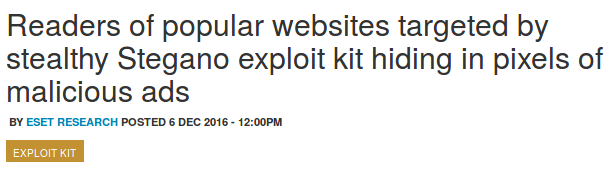
\includegraphics[width=0.9\textwidth]{malvert-stegano}
\end{frame}

\begin{frame}{modern advertising landscape (1)}
    \begin{itemize}
        \item website ads are often \myemph{sold in realtime}
        \item conceptual idea: \myemph{mini-auction} for every ad
        \item major concerns about fraud
            \begin{itemize}
            \item are you really showing my ad?
            \end{itemize}
        \item ad operators want to do own tracking
            \begin{itemize}
            \item get better idea what to show/bid
            \end{itemize}
    \end{itemize}
\end{frame}

\begin{frame}{modern advertising landscape (2)}
    \begin{itemize}
        \item website operators \myemph{typically don't host ads}
            \begin{itemize}
            \item don't build own realtime auction infrastructure
            \item not trusted to report number of ad views correctly
            \end{itemize}
        \item ads often sold indirectly
            \begin{itemize}
            \item middleman handles bidding/etc.
            \item website operators sell to multiple ad operators
            \end{itemize}
    \end{itemize}
\end{frame}

\section{browser exploit mitigations}

\begin{frame}{browsers and exploit mitigations}
    \begin{itemize}
    \item modern browsers employ many of the mitigations we talked about
        \begin{itemize}
        \item full ASLR
        \item write XOR execute (with exceptions for runtime-compiled code)
        \item stack canaries
        \end{itemize}
    \item also some \myemph{other mitigations}
    \end{itemize}
\end{frame}

\begin{frame}{least privilege}
    \begin{itemize}
    \item why can code running for a webpage install software?
    \item \myemph{never} needs to do that
        \vspace{.5cm}
    \item concept: let's run it without those permissions
    \end{itemize}
\end{frame}

\begin{frame}<1>[fragile,label=multiOS]{multi-user OSs}
\lstset{
    language={},style=small,
    moredelim={**[is][\color{red!70!black}]{~in~}{~end~}},
}
\begin{lstlisting}
cr4bd@labunix01:~$ ~in~cp myprogram.exe /bin/ls~end~
cp: cannot create regular file ‘/bin/ls’: Permission denied
\end{lstlisting}
    \begin{itemize}
        \item programs have \myemph{limited privileges}
        \item<2-> OS tracks ``user'' of running every program
        \item<2-> result: malware I installed shouldn't be able to effect other users
        \item<2-> idea 1: reuse this support for web browsers
            \begin{itemize}
            \item webpage should run as ``different user''
            \item malware should only affect web browser?
            \end{itemize}
    \end{itemize}
\end{frame}

\begin{frame}[fragile,label=permEnforce]{permission enforcement}
    \begin{minted}[fontsize=\small]{C}
struct Process {
    int user_id;
    ...
};
int handle_open_system_call(char *filename, ...) {
    Process* currentProcess = GetCurrentProcess();
    File* file = GetFileByFilename(filename);
    if (!file->UserCanAccess(currentProcess->user_id)) {
        return ERROR_PERMISSION_DENIED;
    }
    ...
}
\end{minted}
\end{frame}

\againframe<2>{multiOS}

\begin{frame}{things browsers need}
    \begin{itemize}
    \item what things should browser be able to do?
    \end{itemize}
\end{frame}

\begin{frame}{things browsers need}
    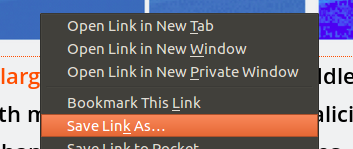
\includegraphics[width=.5\textwidth]{savelinkas}
    \begin{itemize}
        \item save files
        \item have your webmail password
        \item \ldots
    \end{itemize}
\end{frame}

\begin{frame}{the privilege separation idea}
    \begin{itemize}
    \item can't make whole browser run as ``different user''
        \begin{itemize}
        \item still need to save files, read password, etc.
        \end{itemize}
    \item how about just the parts that are ``dangerous''?
        \begin{itemize}
        \item part that runs scripts, parses HTML
        \end{itemize}
    \end{itemize}
\end{frame}

\begin{frame}{simple privilege separation}
    \begin{itemize}
    \item simple example: want to show videos
    \item video decoding library is tens of thousands of lines of code
        \begin{itemize}
        \item often buggy, includes hard-to-check hand-written assembly
        \end{itemize}
    \item what does video decoding library do?
        \begin{itemize}
        \item read video file as input
        \item output images as output
        \end{itemize}
    \end{itemize}
\end{frame}

\begin{frame}{simple privilege seperation}
    \begin{itemize}
    \item setup: create new user
    \item start video decoder as new user
    \item communicate via ``pipes''
        \begin{itemize}
        \item like terminal to be used by program
        \end{itemize}
    \end{itemize}
\end{frame}

\begin{frame}[fragile,label=privSepOutline]{simple privilege seperation}
    \vspace{-.5cm}
\begin{minted}[fontsize=\fontsize{10}{10}]{C}
/* dangerous video decoder to isolate */
int main() {
    /* switch to right user */
    SetUserTo("user-without-privileges"));
    while (fread(videoData, sizeof(videoData), 1, stdin) > 0) {
        doDangerousVideoDecoding(videoData, imageData);
        fwrite(imageData, sizeof(imageData), 1, stdout);
    }
}

/* code that uses it */
    FILE *fh = RunProgramAndGetFileHandle("./video-decoder");
    for (;;) {
        fwrite(getNextVideoData(), SIZE, 1, fh);
        fread(image, sizeof(image), 1, fh);
        displayImage(image);
    }
\end{minted}
\end{frame}

\begin{frame}{issues with privilege separation (1)}
    \begin{itemize}
    \item ``other user'' can still do too much
    \vspace{.5cm}
    \item read unprotected files
        \begin{itemize}
        \item most of them?
        \end{itemize}
    \item write temporary files?
    \item open network connections
    \item use all your memory
    \item \ldots
    \end{itemize}
\end{frame}

\begin{frame}{issues with privilege separation (2)}
    \begin{itemize}
    \item awkward to do
    \item switching users requires special permissions
    \item seperate user for \myemph{each} video decoder, audio decoder, web page renderer?
        \begin{itemize}
        \item users can debug processes from same user
        \end{itemize}
    \item slowdown --- extra copying
    \end{itemize}
\end{frame}

\begin{frame}{recall: process virtual machine}
    \begin{itemize}
    \item process has isolated memory + CPU
    \item communicating outside? needs \myemph{system calls}
        \begin{itemize}
        \item analagous to using I/O devices
        \end{itemize}
    \item \myemph{OS controls what process can do}
    \end{itemize}
\end{frame}

\newmintinline{C}{}

\begin{frame}{Linux system call filtering API}
    \begin{itemize}
    \item privilege seperation support: system call filtering
    \item simple API: \Cinline|seccomp(SECCOMP_SET_MODE_STRICT, 0, 0)|
        \vspace{.5cm}
            \item ``The only system calls the calling thread is permitted to make are \texttt{read},
                \texttt{write}, \texttt{\_exit}, and \texttt{sigreturn}. Other system calls [kill
                the program].''
            \item read/write only work on \myemph{already open files}
    \end{itemize}
\end{frame}

\begin{frame}{``sandboxing''}
    \begin{itemize}
    \item result of filtering called a ``sandbox''
    \item idea: attacker can play in sandbox as much as they want
    \item can't do anything harmful
    \end{itemize}
\end{frame}

\begin{frame}{Chrome architecture}
    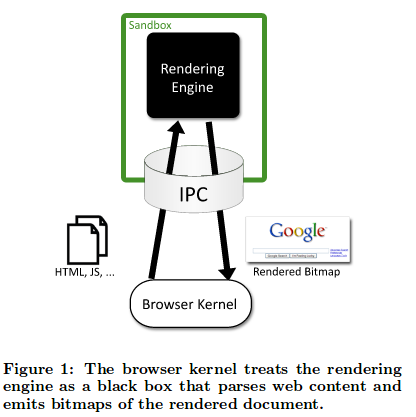
\includegraphics[height=0.8\textheight]{chrome-arch}
\end{frame}

\begin{frame}{talking to the sandbox}
    \begin{itemize}
    \item browser kernel sends commands to sandbox
    \item sandbox sends commands to browser kernel
    \item idea: commands only allow necessary things
    \end{itemize}
\end{frame}

\begin{frame}{original Chrome sandbox interface}
    \begin{itemize}
        \item sandbox to browser ``kernel''
            \begin{itemize}
                \item show this image on screen
                \begin{itemize}
                    \item (using shared memory for speed)
                \end{itemize}
            \item \myemph<2-3>{make request\tikzmark{request} for this URL}
            \item \myemph<4>{download\tikzmark{download} files to local FS}
            \item \myemph<5>{upload\tikzmark{upload} user requested files}
            \end{itemize}
        \item browser ``kernel'' to sandbox
            \begin{itemize}
                \item send user input
            \end{itemize}
    \end{itemize}
    \begin{tikzpicture}[overlay,remember picture]
        \coordinate (middle) at ([yshift=-1cm]current page.center);
        \begin{visibleenv}<2>
            \node[mycallout=request,anchor=center,align=center]  at (middle) {
                needs filtering --- at least no \texttt{file:} (local file) URLs
            };
        \end{visibleenv}
        \begin{visibleenv}<3>
            \node[mycallout=request,anchor=center,align=center] at (middle) {
                can still read any website! \\
                still sends normal cookies!
            };
        \end{visibleenv}
        \begin{visibleenv}<4>
            \node[mycallout=download,anchor=center,align=center] at (middle) {
                files go to download directory only \\
                can't choose arbitrary filenames
            };
        \end{visibleenv}
        \begin{visibleenv}<5>
            \node[mycallout=upload,anchor=center,align=center] at ([yshift=-1cm]middle) {
                browser kernel displays file choser \\
                only permits files selected by user
            };
        \end{visibleenv}
    \end{tikzpicture}
\end{frame}

\begin{frame}<1>{process per site}
    \begin{itemize}
    \item Chrome \myemph{almost} does process-per-site
        \begin{itemize}
        \item idea: one sandbox process per site
        \end{itemize}
    \item with one \myemph{huge exception}
        \begin{itemize}
        \item<2> website one embedded on website two --- still one process
        \end{itemize}
    \item recall: same-origin policy
    \end{itemize}
\end{frame}

\begin{frame}<1>[fragile,label=noSameOrigin]{recall: operations not requiring same origin}
    \begin{itemize}
        \item \myemph<2>{loading images, stylesheets (CSS), video, audio}
        \item \myemph<2>{loading scripts}
        \begin{itemize}
        \item but not getting syntax errors
        \end{itemize}
    \item \myemph<3>{accessing with ``permission'' of other website}
    \item \myemph<4>{submitting forms to other webpages}
    \item \myemph<5>{displaying other webpages} (but not reading contents)
    \end{itemize}
\begin{tikzpicture}[overlay,remember picture]
    \coordinate (overlay) at (current page.center);
    \begin{visibleenv}<2>
    \node[draw,thick,fill=white] at  (overlay) {
        browser kernel checks content-type (sent by server) \\
        doesn't send to sandboxed process if wrong
    };
    \end{visibleenv}
    \begin{visibleenv}<3>
    \node[draw,thick,fill=white] at  (overlay) {
        browser kernel checks headers, \\
        gives content if okay
    };
    \end{visibleenv}
    \begin{visibleenv}<4>
    \node[draw,thick,fill=white] at  (overlay) {
        API to start a sandbox for a different website
    };
    \end{visibleenv}
    \begin{visibleenv}<5>
    \node[draw,thick,fill=white] at  (overlay) {
        not yet implemented by Chrome (by default)? \\
        needs logic to decide where to get images from, etc.
    };
    \end{visibleenv}
\end{tikzpicture}
\end{frame}

\begin{frame}{browser kernel security}
    \begin{itemize}
        \item the browser kernel is not simple
        \item needs to \myemph{securely} implement \myemph{special protocol}
        \item UI, networking code overall more complicated than before
            \vspace{.5cm}
        \item hope: writing secure browser kernel easier than secure whole-browser
    \end{itemize}
\end{frame}

\begin{frame}{OpenSSH privilege seperation}
    \begin{itemize}
    \item OpenSSH uses privilege seperation for its SSH server
    \item what runs on the lab machines when you log into them
    \vspace{.5cm}
    \item separate network processing code from authentication code
    \item seperate process per connection --- users don't share
    \end{itemize}
\end{frame}

\begin{frame}{OpenSSH privsep protocol}
    \begin{itemize}
    \item sandboxed process tells ``monitor'' to:
        \vspace{.25cm}
    \item perform \myemph{cryptographic operations}
        \begin{itemize}
        \item long-term keys never in sandboxed process
        \item commands to ask for cryptographic messages they need
        \end{itemize}
    \item ask to switch to user --- if given user password, etc.
        \begin{itemize}
            \item \myemph{monitor process verifies} login information
        \end{itemize}
    \item after authentication: new process running as logged-in user 
        \begin{itemize}
            \item (normally) no issues with special privileges
        \end{itemize}
    \end{itemize}
\end{frame}


\begin{frame}{privilege seperation overall}
    \begin{itemize}
    \item large application changes
        \begin{itemize}
        \item OpenSSH: 3k lines of code for communication/etc. added
        \item OpenSSH: 2\% of existing code (950 of 44k lines) changed
        \item (but most changes simple)
        \end{itemize}
    \item lots of application knowledge
        \begin{itemize}
        \item what is a meaningful separation of `privileged' and `unprivileged'?
        \end{itemize}
    \item better application design anyways?
    \end{itemize}
\end{frame}

\begin{frame}{application confinement}
    \begin{itemize}
    \item confining whole browsers was hard
        \begin{itemize}
            \item we trust them to do a lot of things --- e.g. write arbitrary files
        \end{itemize}
    \item but maybe we can do this for simpler applications?
    \item idea 1: applications send system calls to OS 
        \begin{itemize}
        \item \myemph{limit syscalls} like we limited browser kernel commands
        \item constructing command language ``in reverse''
        \end{itemize}
    \end{itemize}
\end{frame}

% FIXME: android permissions screen?

\begin{frame}{filtering system calls?}
    \begin{itemize}
    \item example: video player VLC playing a local file on my laptop
    \item uses \myemph{73 unique system calls}
    \item opens many files that \myemph{are not the video file}
        \begin{itemize}
        \item libraries
        \item fonts
        \item configuration files
        \item translations of messages
        \end{itemize}
    \vspace{.5cm}
    \item can I limit the files my video player can read?
    \item how do I come up with a useful filter?
    \end{itemize}
\end{frame}

\begin{frame}{OS X sandboxing}
    \begin{itemize}
    \item OS X (tries to) implement system call filtering
    \item main challenge: what about files?
        \begin{itemize}
        \item user can open a file anywhere --- we expect that to work
        \end{itemize}
    \item<2> OS X solution: OS service displays file-open dialog
        \begin{itemize}
        \item OS knows user really choose a file
        \end{itemize}
    \item<2> application can ask to remember file was chosen previously
    \item<2> not chosen/remembered --- can't access
        \begin{itemize}
        \item requires changes to how applications open files
        \end{itemize}
    \end{itemize}
\end{frame}

\begin{frame}{another sandboxing OS: Qubes}
    \begin{itemize}
    \item Qubes: heavily sandboxed OS
    \item runs \myemph{seperate VMs} instead of filtering syscalls
    \item UI that clearly shows what VM each window is from
    \vspace{.5cm}
    \item advantage: easier to gaurentee isolation
        \begin{itemize}
        \item many, many more bugs in system call filtering than VMs
        \end{itemize}
    \item disadvantage: harder to share between VMs
    \item disadvantage: much more runtime overhead
    \end{itemize}
\end{frame}

\begin{frame}{Qubes screenshot}
    \vspace{-.5cm}
    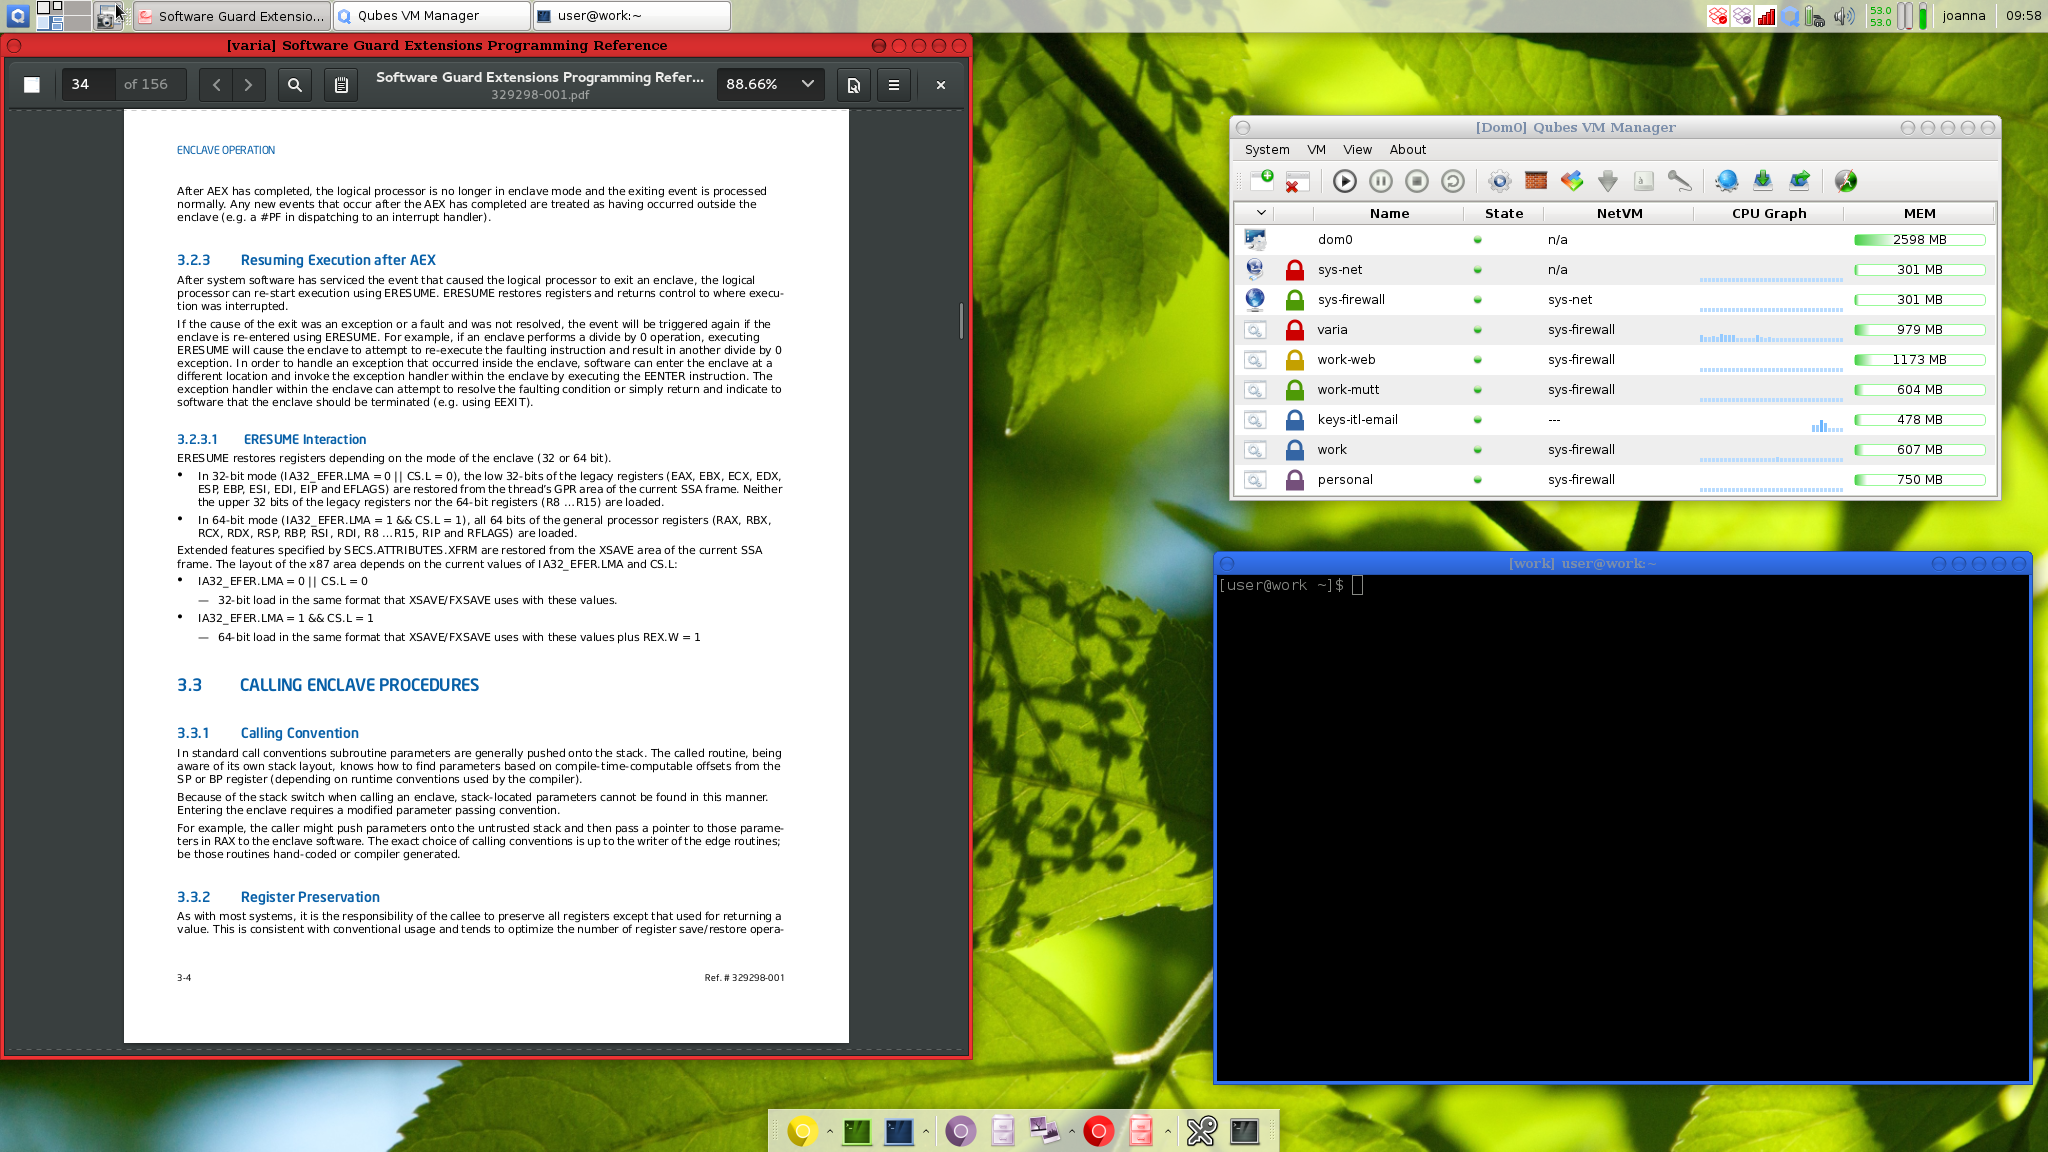
\includegraphics[width=\textwidth]{qubes-desktop1}
\end{frame}


% FIXME: OS X sandboxing weaknesses

% FIXME: Qubes
\begin{frame}{quick review}
    \begin{itemize}
    \item part 1: malware and anti-malware
    \item part 2: (memory) vulnerabilities and exploits and mitigations
    \item part 3: bug-finding/prevention and misc. vulnerabilities and exploits
    \end{itemize}
\end{frame}

\begin{frame}{malware --- evil software}
    \begin{itemize}
        \item tricks itself onto victim machines
            \begin{itemize}
            \item e.g. masquarde as useful software
            \item e.g. embed in legitimate software (viruses)
            \item e.g. attack vulnerabilities in software to spread
            \item e.g. arrange to run automatically on disk insert
            \end{itemize}
        \item cat-and-mouse game --- antivirus software to detect malware
            \begin{itemize}
            \item patterns, heuristics to detect
            \item tricks to appear like normal software
            \end{itemize}
    \end{itemize}
\end{frame}

\begin{frame}{memory vulnerabilities and exploits}
    \begin{itemize}
        \item buffer overflow/underflow --- program writes outside of array
            \begin{itemize}
            \item if ``important'' data, attacker can gain control
            \item usual goal: overwrite pointer to code
            \end{itemize}
        \item use-after-free --- program uses data as wrong type
            \begin{itemize}
                \item attacker controls data as one type
                \item ideally, misinterpreted (via dangling pointer) to contain pointer to code
            \end{itemize}
    \end{itemize}
\end{frame}

\begin{frame}{memory exploit mitigations}
    \begin{itemize}
        \item bounds-checking --- don't allow outside-of-array writes
            \begin{itemize}
            \item doesn't solve use-after-free
            \item single object with array and pointers?
            \end{itemize}
        \item stack canaries --- detect writes next to return addresses
        \item ASLR --- make it so program can't make up useful pointers?
            \begin{itemize}
            \item problem: memory bugs can print out pointers
            \end{itemize}
        \item W xor X --- make it so attacker can't write new code
            \begin{itemize}
            \item problem: attack can reuse existing code (return-oriented programming)
            \end{itemize}
    \end{itemize}
\end{frame}

\begin{frame}{bug-finding}
    \begin{itemize}
        \item systematic testing --- find crashes ($\approx$ vulnerability)
            \begin{itemize}
            \item fuzz testing --- generate random tests
            \item coverage-guided fuzz-testing --- random tests, weighted by what runs
            \item symbolic execution --- solve for input to reach each possibility
            \end{itemize}
        \item static analysis --- look for dangerous patterns
            \begin{itemize}
            \item usually false positives and/or negatives
            \item typically examine potential paths through program
            \end{itemize}
    \end{itemize}
\end{frame}

\begin{frame}{bug-prevention}
    \begin{itemize}
        \item ownership --- enforceable rule to prevent use-after-free
            \begin{itemize}
            \item never free while object is owned
            \item one writer (could be changing internal pointers) or many readers
            \item readers and writers can borrow from owner
            \item language (e.g. Rust) can track borrowing lifetimes to make safe
            \end{itemize}
        \item alternate safe policies --- reference counting, etc.
            \begin{itemize}
            \item have runtime overhead, but can be used only when needed
            \end{itemize}
        \item escape hatch --- only check small amount of unsafe code
            \begin{itemize}
            \item ideally implements policies that make sense
            \item at least limits the code one needs to check
            \end{itemize}
    \end{itemize}
\end{frame}

\begin{frame}{command injection/web security}
    \begin{itemize}
        \item command injection --- type confusion problems
            \begin{itemize}
            \item try to embed constant/etc., end up embedding commands
            \item lots of languages to embed in --- command line, SQL, HTML, \ldots
            \end{itemize}
        \item web security
            \begin{itemize}
                \item same origin policy (SOP) --- isolate by domain name (mostly)
            \item XSS --- command injection for the web
            \item trusting client inputs --- the attacker controls their browser
            \item CSRF --- innocent browser submits bad request (w/ cookies) for attacker
            \item clickjacking --- ``steal'' user's click to make request
            \end{itemize}
    \end{itemize}
\end{frame}


\begin{frame}{next time}
    \begin{itemize}
    \item final exam review: bring questions
    \end{itemize}
\end{frame}


